%% ----------------------------------------------------------------
%% Thesis.tex -- MAIN FILE (the one that you compile with LaTeX)
%% ----------------------------------------------------------------

% Set up the document
\documentclass[a4paper, 11pt, oneside]{Thesis}  % Use the "Thesis" style, based on the ECS Thesis style by Steve Gunn
\graphicspath{Figures/}  % Location of the graphics files (set up for graphics to be in PDF format)

% Include any extra LaTeX packages required
\usepackage[square, numbers, comma, sort&compress]{natbib}  % Use the "Natbib" style for the references in the Bibliography
\usepackage[nottoc]{tocbibind} % bind bibliography to the table of contents
\usepackage{verbatim}  % Needed for the "comment" environment to make LaTeX comments
\usepackage{vector}  % Allows "\bvec{}" and "\buvec{}" for "blackboard" style bold vectors in maths
\usepackage[table]{xcolor}
\usepackage{array, tabularx, caption, boldline}
\usepackage{float}
\hypersetup{urlcolor=black, colorlinks=true}  % Colours hyperlinks in black, can be distracting if there are many links and colored blue.

%% ----------------------------------------------------------------
\begin{document}
\frontmatter      % Begin Roman style (i, ii, iii, iv...) page numbering

% Set up the Title Page
\title  {Supervised \& Unsupervised Learning Methods to Produce Consumer Energy Profiles}
\authors  {Niall Trinder}

\addresses  {\groupname\\\deptname\\\univname}  % Do not change this here, instead these must be set in the "Thesis.cls" file, please look through it instead
\date       {\today}
\subject    {}
\keywords   {}

\maketitle
%% ----------------------------------------------------------------

\setstretch{1.3}  % It is better to have smaller font and larger line spacing than the other way round

% Define the page headers using the FancyHdr package and set up for one-sided printing
\fancyhead{}  % Clears all page headers and footers
\rhead{\thepage}  % Sets the right side header to show the page number
\lhead{}  % Clears the left side page header

\pagestyle{fancy}  % Finally, use the "fancy" page style to implement the FancyHdr headers

%% ----------------------------------------------------------------
% Declaration Page required for the Thesis, your institution may give you a different text to place here
\Declaration{

\addtocontents{toc}{\vspace{1em}}  % Add a gap in the Contents, for aesthetics

I, Niall Trinder, declare that this thesis titled, `Supervised \& Unsupervised Learning Methods to Produce Consumer Energy Profiles?' and the work presented in it are my own. I confirm that:

\begin{itemize}
\item[\tiny{$\blacksquare$}] This work was done wholly or mainly while in candidature for an undergraduate degree at Cork Institute of Technology.

\item[\tiny{$\blacksquare$}] Where any part of this thesis has previously been submitted for a degree or any other qualification at Cork Institute of Technology or any other institution, this has been clearly stated.

\item[\tiny{$\blacksquare$}] Where I have consulted the published work of others, this is always clearly attributed.

\item[\tiny{$\blacksquare$}] Where I have quoted from the work of others, the source is always given. With the exception of such quotations, this project report is entirely my own work.

\item[\tiny{$\blacksquare$}] I have acknowledged all main sources of help.

\item[\tiny{$\blacksquare$}] Where the thesis is based on work done by myself jointly with others, I have made clear exactly what was done by others and what I have contributed myself.
\\
\end{itemize}


Signed:\\
\rule[1em]{25em}{0.5pt}  % This prints a line for the signature

Date:\\
\rule[1em]{25em}{0.5pt}  % This prints a line to write the date
}
\clearpage  % Declaration ended, now start a new page

%% ----------------------------------------------------------------

% The Abstract Page
\addtotoc{Abstract}  % Add the "Abstract" page entry to the Contents
\abstract{
\addtocontents{toc}{\vspace{1em}}  % Add a gap in the Contents, for aesthetics

Currently in developed nations, building energy consumption makes up approximately 39\% of primary energy consumption ~\cite{energy2011building}. As we see dense urban areas continue to grow and spread, one stand out opportunity looking forward for the energy sector is energy demand forecasting.\\
\indent In recent times, approaches to data analytics have been adopted in almost every aspect of society. As this adoption continues we see new methodologies being developed in order to deal with the ever-increasing quantity of data being generated. The challenge of capturing, storing and processing extraordinary large volumes of data is commonly referred to as big data. A major challenge of this paradigm is our ability to perform an analysis and extract meaningful insights from big data in any sort of time sensitive situations. This requires intelligent and innovative solutions to overcome these challenges. This dissertation explores the issues surrounding this challenge and identifies the opportunities to be realised using new technologies to identify valuable insights in consumption patterns. 

}

\clearpage  % Abstract ended, start a new page
%% ----------------------------------------------------------------

\setstretch{1.3}  % Reset the line-spacing to 1.3 for body text (if it has changed)

% The Acknowledgements page, for thanking everyone
\acknowledgements{
\addtocontents{toc}{\vspace{1em}}  % Add a gap in the Contents, for aesthetics

The acknowledgements and the people to thank go here, don't forget to include your project adviser\ldots

}
\clearpage  % End of the Acknowledgements
%% ----------------------------------------------------------------

\pagestyle{fancy}  %The page style headers have been "empty" all this time, now use the "fancy" headers as defined before to bring them back


%% ----------------------------------------------------------------
\lhead{\emph{Contents}}  % Set the left side page header to "Contents"
\tableofcontents  % Write out the Table of Contents

%% ----------------------------------------------------------------
\lhead{\emph{List of Figures}}  % Set the left side page header to "List if Figures"
\listoffigures  % Write out the List of Figures

%% ----------------------------------------------------------------
\lhead{\emph{List of Tables}}  % Set the left side page header to "List of Tables"
\listoftables  % Write out the List of Tables

%% ----------------------------------------------------------------
\setstretch{1.5}  % Set the line spacing to 1.5, this makes the following tables easier to read
\clearpage  % Start a new page
\lhead{\emph{Abbreviations}}  % Set the left side page header to "Abbreviations"
\listofsymbols{ll}  % Include a list of Abbreviations (a table of two columns)
{
% \textbf{Acronym} & \textbf{W}hat (it) \textbf{S}tands \textbf{F}or \\
\textbf{LAH} & \textbf{L}ist \textbf{A}bbreviations \textbf{H}ere \\

}


%% ----------------------------------------------------------------
\mainmatter	  % Begin normal, numeric (1,2,3...) page numbering
\pagestyle{fancy}  % Return the page headers back to the "fancy" style

% \usepackage{listings}
\chapter{Introduction}
\lhead{\emph{Introduction}}
This section will introduce the thesis.
\section{Smart Grids}
The energy grid is comprised of four main sectors:

        \begin{center}
            \begin{tabular}{|l |l|}
            \hline
             \textbf{Sector} & \textbf{Description} \\
             \hline\hline
             \hline
             Generation & 
             Energy is produced through either renewable or non-renewable \\ &
             sources, for example a coal burning power plant or a hydro-electric \\  &
             power producing dam. \\
             \hline
             Transportation & 
             Energy which has been produced is transmitted in high volume from \\ &
             the point of origin towards the something dense regions \\ &
             where the energy is consumed. \\
             \hline
             Distribution & 
             The power is redistributed to where the load is required along \\ &
             a local network connected to the end consumers. \\ 
             \hline
             Consumption & 
             Where the energy is consumed by the end user. \\
             \hline
            \end{tabular}
        \end{center}
In traditional power grids, the power generation comes from large centralized facilities. The power is then sent to central load centres which then directly sends power to the consumers as load requires. In a smart grid there is an unconventional power flow, meaning that the flow of power can be managed in order to redistribute it. It supports a two-way flow of information, being that utilities can send commands to the consumer as well as the end user is capable of gathering and returning information on their power consumption back to the utility. Smart grids allow for a automatic \& distributed energy delivery network.
A smart meter is a device installed on the consumer end of the energy grid. It is an advanced digital energy meter which contains information from the end user's load devices. It's capable of measuring the energy consumption of the consumer in real time. The information gathered by the smart meter can be transmitted back to the utilities. In the existing grid system, consumption monitoring is carried out manually which delays the billing process and doesn't allow for consumers to make smart decisions around their energy consumption such as using energy heavy devices during peak load times when energy is at a premium. Smart meters allow for real time consumption monitoring and automatic billing. As the communication between user and utility is bi-directional, the utility can now remotely disconnect and reconnect loads. In addition to real time monitoring, utility companies can use the data gathered to construct models to accurately forecast demand.  You can break down energy forecasting into three categories, short, medium and long term. Short term demand modelling is used to forecast energy consumption hours or days in advance. This provides valuable maintenance and operation information, for example this will determine how which power producing facilities will be required to be online for a certain time period. This type of forecasting has obvious environmental impacts as it allows energy producers to minimize the number of non-renewable power producing facilities to be active and maximizes the number of renewable power sources. Medium term forecasting is of particular interest to energy companies as it provides them with information about the market needs of energy moving forward, this will allow them to schedule fuel prices and reduce financial risk. Long term forecasting is important on a governmental level, allowing for policy makers to plan ahead. A smart meter's data could be built up of a unique identification, the electrical consumption (typically in kWh for domestic dwellings) and a time stamp. Other data can be sent back to the utility in order to diagnose detected anomalies. Value propositions for the various stakeholders. 
%https://ieeexplore-ieee-org.cit.idm.oclc.org/document/1717600
\begin{itemize}
\item The Utilities
    \begin{itemize}
    \item It saves a lot of money by improving the remote area reading and billing system
    \item It gives the ability to better manage during peak load times
    \item It makes more efficient use of energy grid resources
    \item It offers new tariff model in the electricity market
    \item It improves the transformer load management for the transmission lines
    \end{itemize}
\item The Consumers
    \begin{itemize}
    \item It shows customer data about their electricity habit
    \item It gives customer more accurate timely electricity billing
    \item It helps customer to better use the electrical equipment during the expensive hours
    \item It facilitates customer to switch/delay their electrical equipment with significant consumption to less expensive hours
    \end{itemize}
\item Governments
    \begin{itemize}
    \item It stimulates the economy by investing in smart metering networks
    \item It improves the environmental condition by reducing C02 emission
    \item It leads to reduction of consumption by increasing the awareness of consumption pattern
    \item It gives data for improving efficiency and reliability of service
    \end{itemize}
\end{itemize}

Means of generating and storing user data has evolved greatly over the past number of years, for example, through smart metering its possible to install a device to monitor and store the energy consumption of a domestic or residential property on a minute by minute basis. \\
Typically in residential setting, an analogue energy meter is installed in the premises. This meter reads the amount of energy consumed in kWh. Energy suppliers will typically send out  a technician to take a reading which then can be billed back to the consumer. In the interim between technician visits, the energy supplier could make an estimate of the energy consumption based on previous readings. Smart metering allows for the streaming of data back to the energy supplier. This removes the need for the energy supplier to schedule routine inspections. There is a big drive from Utility companies to upgrade their infrastructure and integrate more advanced tools for monitoring consumer behaviour.
For instance, the energy sector is moving towards an Intelligent Energy Network (IEN), the goal of IENs is to enable reliable, stable, secure and smart energy networks. These way this can be achieved is through incorporating new technologies and through higher integrating between existing services. There are many different focus areas of an IEN such as energy storage integration, Protection and fault calculation, Stability, Reliability \& Power quality to name a few.

%https://www.et.aau.dk/research-programmes/intelligent-energy-systems-and-active-networks/mission-and-focus-areas/ \\
% **HERE: What do we aim to do?**


        \begin{figure}[H]
        \centering     
        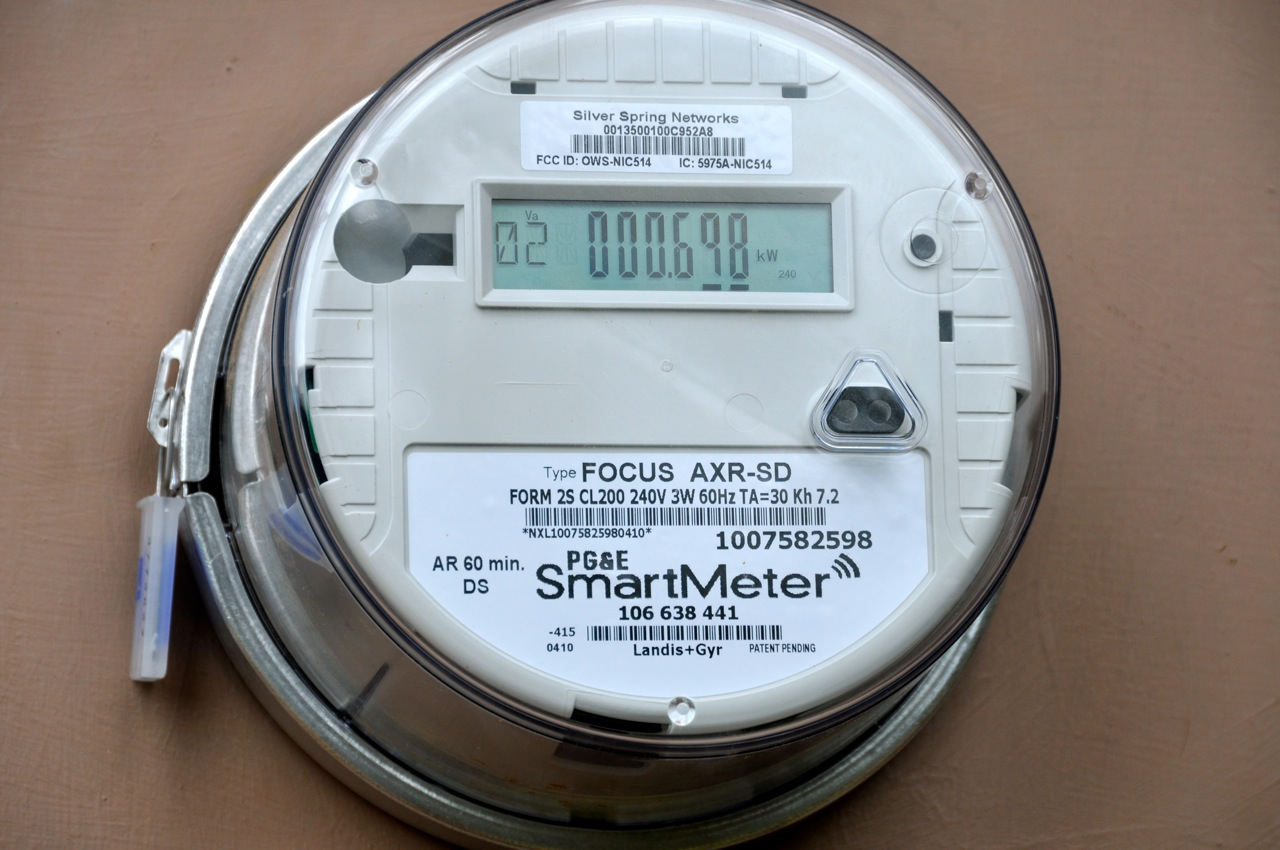
\includegraphics[width=1\textwidth]{Figures/smart-meter-emf-safety-network.jpg}
        \caption{Example of a Smart Meter}
        \label{fig:Daily Consumption}
        \end{figure} % Introduction

\chapter{Literature Review}
\section{Introduction}
In this chapter, each of the elements of the work flow outlined in this project are discussed with relation to work published in similar areas. The areas of particular focus are data pre-processing, unsupervised learning and supervised learning. Each section will outline and explain certain concepts covered in this thesis and also look at papers with similar challenges.
\lhead{\emph{Background}}
\section{Data Pre-processing}
Data pre-processing is the work done to transform a data-set prior to applying any machine learning algorithms. On a basic level, different algorithms require different structures to the data in order to compile. An example of this is some algorithms handling missing data poorly so often the data points with missing values are investigated and either removed or imputed. There are many other potential roadblocks that can prevent an algorithm from working such as correct date formatting, there are also another set of operations which transform the existing data in order to increase the performance of the model. For instance removing outliers, normalizing the data set or accounting for seasonal difference will all help towards improving the accuracy of the model. Depending on the data set and the aim of the model, the steps taken in the data pre-processing can vary. Models that work with word processing will have to tokenize the words and count the frequency, some data sets containing variables such as gender or colour are transformed into dummy variables which represent categorical variables as binary variables.

\\


\section{Unsupervised Learning}
\subsection{Clustering}
Clustering is a solution for classifying and labelling data into distinct classes when there is no prior knowledge about the existence of these classes, this is referred to as unsupervised classification. This project will analyse energy consumption data of domestic consumers measured on a 30 minute time resolution over the period of 2 years. The initial goal is to partition the consumers based on habitual behaviour in order to develop energy consumption profiles, the role of clustering becomes clear. \\
Clustering is the process of taking $n$ number of data points and fitting them to $j$ number of disjointed clusters. In this scenario, all data points within an individual cluster are similar however each cluster is distinct from any other. There are numerous techniques used for unsupervised clustering, one of which is $k$-means clustering, favoured by virtue of being one of the more straight forward techniques available ~\cite{KMC}. $k$-means clustering finds the partition of the data given $n$ number of observations into $k (\leq n)$ sets $S = \{S_1,S_2, \dots, S_k\}$ so as to minimize the within-cluster sum of squares. This can be represented as the following:

\begin{equation}
\stackrel{arg min}{_{S}} \sum_{i=1}^k \sum_{x \epsilon S_{i}} \Vert x-\mu_{i} \Vert ^{2} = \stackrel{arg min}{_{S}}  |S_{i}|  Var S_{i}
\end{equation}
Where $\mu_{i}$ is the mean of points in $S_i$. This is equivalent to minimizing the pairwise squared deviations of points in the same cluster:
\begin{equation}
\stackrel{arg min}{_{S}} \sum_{i=1}^k \frac{1}{2|S_i|} \sum_{x, y\epsilon S_i}\Vert x- y \Vert ^2
\end{equation}
A limitation of the $k$-means is that it is only optimal for spherical clusters. The clusters are to be expected to be of equal or similar size which may not always be the case. There are other models available such as the Gaussian models which are more flexible by having both variances and covariances.

One common method used to predict or monitor future values for time series data is classification methods which assign a category to patterns in the series. 

\subsection{Hierarchical Clustering}
Similarity or dissimilarity is a method by which a data set can be partitioned based on the distance between static objects . There are different distance measurements designed for specifying similarity between time-series. Hausdorff distance, modified Hausdorff (MODDH) HMM-based distance, Euclidean distance, Euclidean distance in a PCA subspace, and Longest Common Sub Sequence (LCSS) are the most popular distance measurement methods that are used for time-series data \cite{AGHABOZORGI201516}.\\
In building energy profiles, for balanced general solutions, Euclidean distance is the measure that obtains the best results. Dynamic Time Warping (DTW) distance can be regarded as an improved alternative distance measurement over Euclidean distance in applications that make the most of better representation of the high-similar nuclei and where losing capabilities to capture and average the no-so-similar samples is not a critical factor ~\cite{8581840920130201}.\\

\subsection{Distance Measurement MPdist}
As mentioned above, Euclidean Distance and Dynamic Time Warp (DTW) have been accepted into the community as two effective measurement distances but these measures are not without fault as we can see in ~\cite{Gharghabi2018AnUT}. Shaghayegh et al. introduces a new measure called MPdist, the advantage of this measurement is being able to handle missing values or spurious regions. Additionally using this measurement over the Euclidean or DTW measures increases computation efficiency. In the field of energy consumption where a huge amount of data is continually generated, this is advantages as it allows for analysis on larger quantities of data streams. Some necessary definitions must be outlined before defining the MPdist formula as found in ~\cite{Gharghabi2018AnUT}.\\


\textbf{Definition 1:} A Time Series T = $t_1, t_2, \dots, t_n$ is a sequence of $n$ real values. MPdist is a distance measurement between two time series.\\
\textbf{Definition 2:} A subsequence T$_{i,L}$ is a contiguous subset of values with length $L$ starting from position $i$ in the time series T. The subsequence T$_{i,L}$ is in the form T$_{i,L} = t_i, t_{i+1},\dots, t_{i+L-1}$ where $1 \leq L \leq |T|$\\
\textbf{Definition 3:} Sliding window. All possible subsequences of a given time series T can be extracted by sliding a window of size $L$ across T. There are ($n - L + 1$) such subsequences, which we denote as $SubseqNum$.\\
At a high level, the proposed MPdist measurement will compute the distance between two time series T$_A$ and T$_B$, by aggregating the distances between All-subsequences set. For this purpose, we need to find the nearest neighbor for each subsequence in A within B (and visa versa). To determine if a member of set B is the nearest neighbor of a member in set A we use 1NN-Join Function.\\
\textbf{Definition 4:} An All-Subsequences Set A is a set of all possible subsequences of a time series T. The subsequences are obtained from sliding a window of length $L$ across T. Thus,\\
\begin{equation}
A = \{T_{1,L}, T_{2,L},\dots, T_{n-L+1,L}\}
\end{equation}\\
\textbf{Definition 5:} 1NN-Join Function is defined as the first nearest neighbor (1NN) between two subsequences A[$i$] and B[$j$].\\
The 1NN-join function is a similarity join operator, which is applied on two All-subsequence sets, as a result we can create the AB similarity set:\\
\textbf{Definition 6:} AB Similarity Join J$_{AB}$ is a set containing pairs of each subsequence in A with its corresponding nearest neighbor in B. In which A and B are two sets of All-subsequences. $J_{AB}$ is defined as:
\begin{equation}
J_{AB} = \{\langle A[i], B[j]\rangle \; | \; \theta_{1NN}(A[i], B[j])\}
\end{equation}\\
The similarity join set contains tuples, with each subsequence in a set A from the time series T$_A$, and its nearest neighbor in set B from time series T$_B$. Note that some subsequences in T$_B$ may not be used as neighbors to any elements from T$_A$, and some subsequences in T$_B$ may be used more than once. This is because in general $J_{AB} \neq J_{BA}$.\\
For the proposed MPdist distance measure, we need to obtain the distance between each pair in the similarity join set. After obtaining the nearest neighbor of each subsequence in a set, an array which stores the Euclidean distance of each pair is called the Matrix Profile.\\
\textbf{Definition 7:} Matrix Profile P$_{AB}$ is an array in which the Euclidean distance between each pair in $J_{AB}$ is stored. The length of $P_{AB}$ is ($n - L + 1$) or $SubseqNum$. \\
Without loss of generality, it is assumed that the two time series T$_A$ and T$_B$ have the same length. Moreover, it rarely makes sense to measure the similarity of time series with significantly different lengths.\\
Fig. 2.1 shows the $P_{AB}$ of two time series T$_A$ and T$_B$. As shown, since T$_A$ and T$_B$ have most common structure, their P$_AB$ has low values except for the region where sine-waves change to triangular wave, in which case there is no "explanation" from T$_{B}$ in T$_{A}$, hence, there is a bump in P$_{AB}$ indicating a high value.

\begin{figure}
\centering     
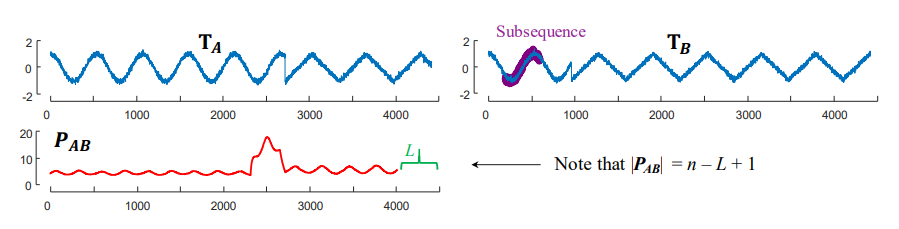
\includegraphics[width=1\textwidth]{Figures/MPdist_fig3.png}
\caption{(top) Two time series T$_A$ and T$_B$, (bottom) P$_{AB}$ of two time series T$_A$ and T$_B$ with $L = 400$. Because there is no corresponding section in T$_A$ from T$_B$ at the point of signal change, there is a bump in P$_{AB}$}
\label{fig:MPdist}
\end{figure} 

The time complexity to calculate P$_{AB}$ for two equal-length time series with $L$ is much shorter than $n$ is $O(n^2)$. If the length of $L$ is a significant fraction of $n$, then the time complexity grows to $O((n - L + 1) \times n)$. In the limit, when $L = n$, this degenerates to the special case of Euclidean distance between two time series, which takes $O(n)$. The following notation summarizes this:

\begin{equation}
\textrm{Time complexity } P_{AB} = \Bigg\{ \substack{
O(n^2)\ \\
O((n - L + 1) \times n), \\
O(n),
}
\substack{
L \ll n \\
L < n \\
L = n}
\end{equation}

As $L$ approaches $n$, the time complexity approaches linear time. To make this distance measure between T$_A$ and T$_B$ symmetric, both J$_{AB}$ and J$_{BA}$ need to be computed. This is denoted as the ABBA similarity join:

\textbf{Definition 8: } ABBA Similarity Join J$_{ABBA}$ is a set containing pairs of subsequence in A with its nearest neighbor in B and vice versa.\\
Note that if a subsequence in A (denoted as T$_{A,i}$) is the nearest neighbor of a subsequence in B (denoted as T$_{B,j}$) the reverse of that may not be true. An array which stores all distances in ABBA similarity join set is Join Matrix Profile:
\\
\textbf{Definition 9: }Join Matrix Profile P$_{ABBA}$ is an array contain the Euclidean distance for each pair in J$_{ABBA}$. The length of the P$_{ABBA}$ is $2 \times (n - L) + 2$ which is twice the length of P$_{AB}$.
\\
The  matrix profile has distances for both similarity joins J$_{AB}$ and J$_{BA}$, thus it is symmetric in terms of the order of the time series. As a result, the distance calculated based on J$_{ABBA}$ between T$_{A}$ and T$_{B}$ is also equal. Fig. 2.2 shows an illustration of the P$_{ABBA}$ of two time series T$_{A}$ and T$_{B}$.

\begin{figure}
\centering     
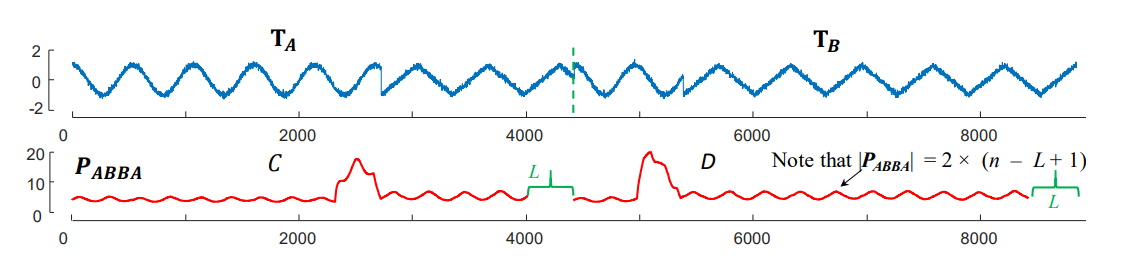
\includegraphics[width=1\textwidth]{Figures/MPdist_fig4.png}
\caption{(top) The concatenation of two time series T$_A$ and T$_B$, (bottom) P$_{ABBA}$ of two time series T$_A$ and T$_B$ with $L = 400$. The distance between each subsequence from T$_A$ and its nearest neighbor from T$_B$ is calculated in C and the reverse in D. There is a gap between C and D at the middle, because the length of the remaining data in T$_A$ is less than the subsequence length thus, the distance cannot be calculated.}
\label{fig:MPdist}
\end{figure} 

The MPdist formula is as follows:

\begin{equation}
MPdist = \Bigg\{ 
\stackrel 
    {k^{th} \textrm{value of sorted} P_{ABBA}}
    {max(P_{ABBA}),}
\qquad 
\stackrel
    {|P_{ABBA}| > k}
    {|P_{ABBA}| \leq k}
\end{equation}

The worse case complexity of MPdist is $O(n^2)$ which would make it unsuitable for large datasets.However as shown in ~\cite{Gharghabi2018AnUT}, the complexity can be reduced to $O(m \times SubseqNum)$ time.



\subsection{Fuzzy Logic}
There is scope here to introduce fuzzy logic, as  Maharaj et al. outline ~\cite{MAHARAJ20111187}, fuzzy logic allows a non-strict representation of object membership to a set. These membership grades indicate the degree to which the data points belong to each cluster. In conventional clustering techniques data points right on the boundary of a cluster hold the same relationship to the cluster as those in the very centre. Using the membership grade, these points at edge of the cluster can still be inside the cluster but to a lesser degree than those at its centre. This may be necessary due to imprecise and uncertain data introduced through for example, faulty monitoring equipment. Fuzzy k-means is a clustering method that has proved effective in many scenarios since it permits the assignment of data elements to one or more clusters ~\cite{MOLINASOLANA2017598}. Fuzzy logic is based on minimization of the following objective function:

\begin{equation}
J_m = \sum_{i=1}^{n} \sum_{j=1}^{c} u_{ij}^{m} \Vert x_i - c_j \Vert  \qquad  \textrm{for}   \quad i \leq m < \infty
\end{equation}

where, membership:
\begin{equation}
u_{ij} = \frac{1}{\sum_{k=1}^c (\frac{\Vert x_i - c_j \Vert}{\Vert x_i - c_k \Vert})^ \frac{2}{m-1}}
\end{equation}\\
cluster centres:
\begin{equation}
c_j = \frac{\sum_{i=1}^n u_{ij}^m . x_i}{\sum_{i=1}^n u_{ij}^m}
\end{equation}

%https://www-sciencedirect-com.cit.idm.oclc.org/science/article/pii/S0020025510005840 \\
%https://home.deib.polimi.it/matteucc/Clustering/tutorial_html/cmeans.html

Here, $m$ is the fuzzy parameter taking on any real number greater than 1. Values too close to 1 will result in a hard border like partition with all membership values close to 0 or 1. Large values of $m$ will result in homogeneous membership values close to $1/c$ ($c$ number of clusters). As such, neither values are used. In practice the most popular choice for the fuzzy parameter is $m = 2$, Hwang et al. chose $m = 2$ for their chosen model ~\cite{hwang}, as do Yang et al. in theirs ~\cite{4522596}. \\

% ADD THESE REFERENCES
%https://www-sciencedirect-com.cit.idm.oclc.org/science/article/pii/S0020025510005840\\
%https://link.springer.com/article/10.1007/s11336-005-1314-x \\
%https://books.google.ie/books?hl=en&lr=&id=z6XqBwAAQBAJ&oi=fnd&pg=PR14&ots=0h-OpWEnDr&sig=anHAa-7nUJzQURPcZcs4gABJUho&redir_esc=y#v=onepage&q&f=false \\ 
%https://ieeexplore.ieee.org/abstract/document/4522596 \\

Additionally, $u_{ij}$ is the degree of membership of $x_i$ in the cluster $j$ $x_i$ is the $i$th d-dimensional measured data, $c_j$ is the d-dimensional centre of the cluster, and $\Vert * \Vert$ is any norm expressing the similarity between any measured data and the centre.

% ADD THESE REFERENCES
%https://www-sciencedirect-com.cit.idm.oclc.org/science/article/pii/S0031320310003973 % Literature Review

\chapter{Methodology}
As outlined in the introduction, we seek to find out if we can use consumer energy time series data to identify clusters of consumption patterns and can we use geographic and demographic data about those consumers to predict which cluster a consumer belongs to. In order to answer this question we're going to look at ways and methods to read in a large time series data file and perform clustering techniques to discover distinct groups based on energy consumption. We then will look at ways in which to use accompanying geographic and demographic data to classify a consumer into one of the distinct energy clusters.

\section{Description of Data}
    The data available was sourced from the UK Data Archive, Study Number 7591 - Energy Demand Research Project: Early Smart Meter Trials, 2007-2010. It contains the following:
    \subsection{Smart Meter Electrical Energy Consumption Readings}
        \subsubsection{Description of Variables}
    
            \\
            This file is in a CSV format. The electrical energy consumption file contains 413,836,038 readings in total for 14,621 households with a total disk space of 12GB. There are 4 variables, the description of each can be found in the accompanying documentation: 
        \begin{center}
            \begin{tabular}{|l | l|}
            \hline
             \textbf{Variable Name} & \textbf{Description} \\
             \hline\hline
             ANON\_ID & Integer case identifier (unique, not null, use to \\&  link records in the other files) \\ 
             \hline
             ADVANCEDATETIME & Date-Time of electricity read (half-hour precision) \\
             \hline
             HH & Half-hour indicator for each day (1-48) \\
             \hline
             ELECHKWH & Unit of kilowatt-hours consumed in that half-hour \\
             \hline
            \end{tabular}
        \end{center}
        
        \subsubsection{Exploratory Data Analysis on Consumption Data Set}
        Performing Exploratory Data Analysis (EDA) provides valuable insights, it introduces the data set and describes the data being studied. This data set contains the energy consumption measured by smart meters (in kilowatt-hours) starting at midnight and taking measurements every half-hour onwards. This is a classic example of a time-series data set with $key:value$ entries. Here our key is the time stamp at which a reading was taken (ADVANCEDATETIME) and the value is the consumption amount (ELECKWH). In addition to this we have the device identification (represented as ANON\_ID), we discuss how the data is to be structured in a future section, 3.3.2. This section will focus on carrying out EDA on a time period partition (or epoch) of the data set from the first 'chunk' of data which relates to the first 100,000 entries in the data set. 
        
        \begin{figure}[H]
        \centering     
        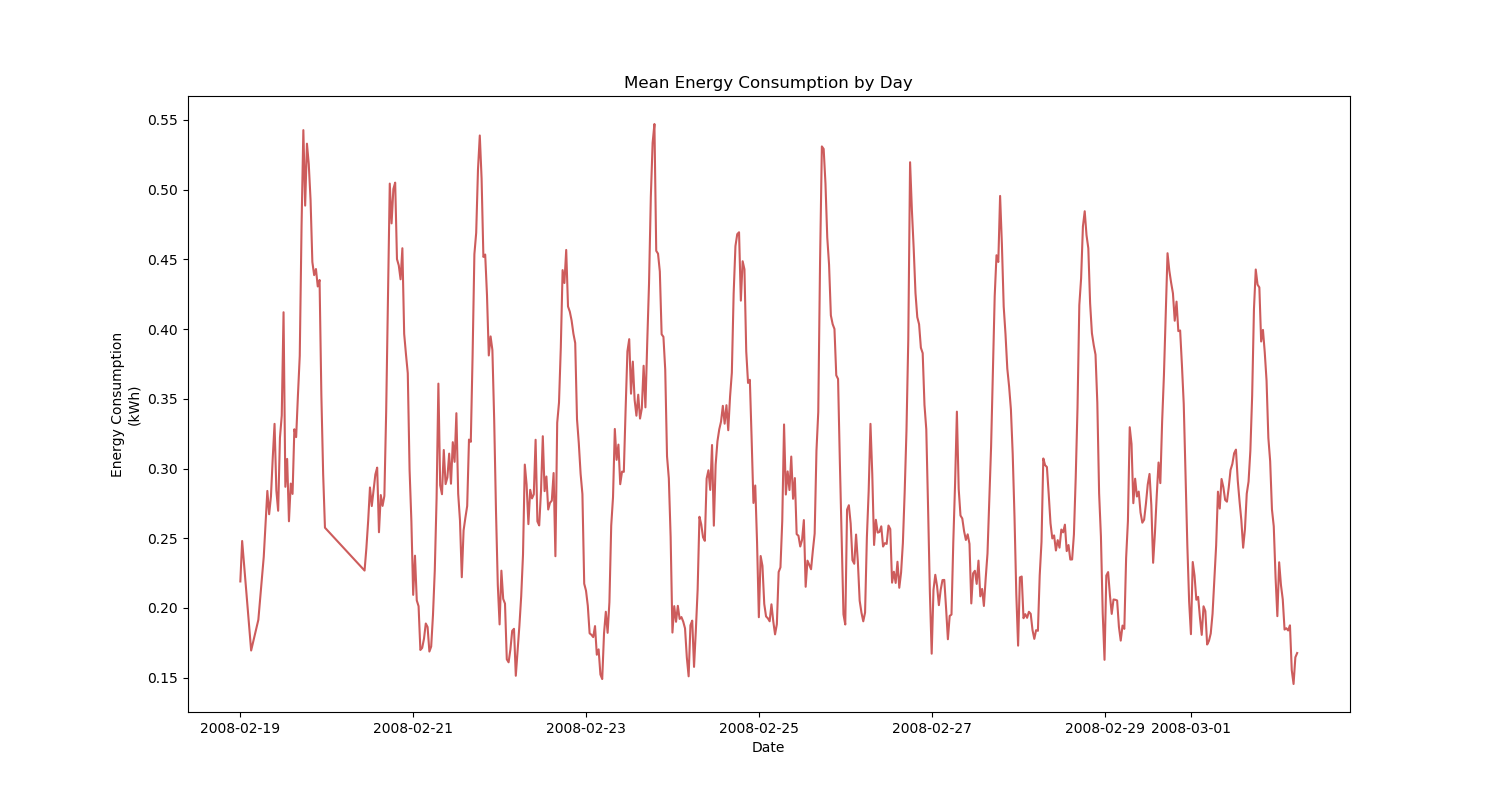
\includegraphics[width=1\textwidth]{Figures/EDA_images/mean_consumption_day.png}
        \caption{Mean Consumption for All Meters}
        \label{fig:Mean Consumption}
        \end{figure} 
        
        Figure 3.1 shows the mean consumption of energy across all devices for 12 day period.  Here we can see the huge variation in load on a daily basis. There appears to be a clear daily trend with a peak at some point during the day, a low point at some point and a period of medium energy consumption in between. To further investigate the daily cycle of energy consumption, fig.3.2. shows the mean energy consumption of a 24 hour period on a half-hourly resolution from the data set. Here we see the period between midnight and 5am has the lowest half-hour energy consumption with approx 0.2kWH consumed every 30 minutes per smart meter. This has significant importance to energy providers as this corresponds to the minimum amount of energy that has to be produced 24/7. After 5am a step incline in energy consumption can be observed, from 0.2 kWH to 0.3 kWh, which then holds consistently until approx 3pm. After 3pm we again see a further step incline to a peak of ~0.48 kWh just before 8pm before falling off dramatically.
        
        \begin{figure}[H]
        \centering     
        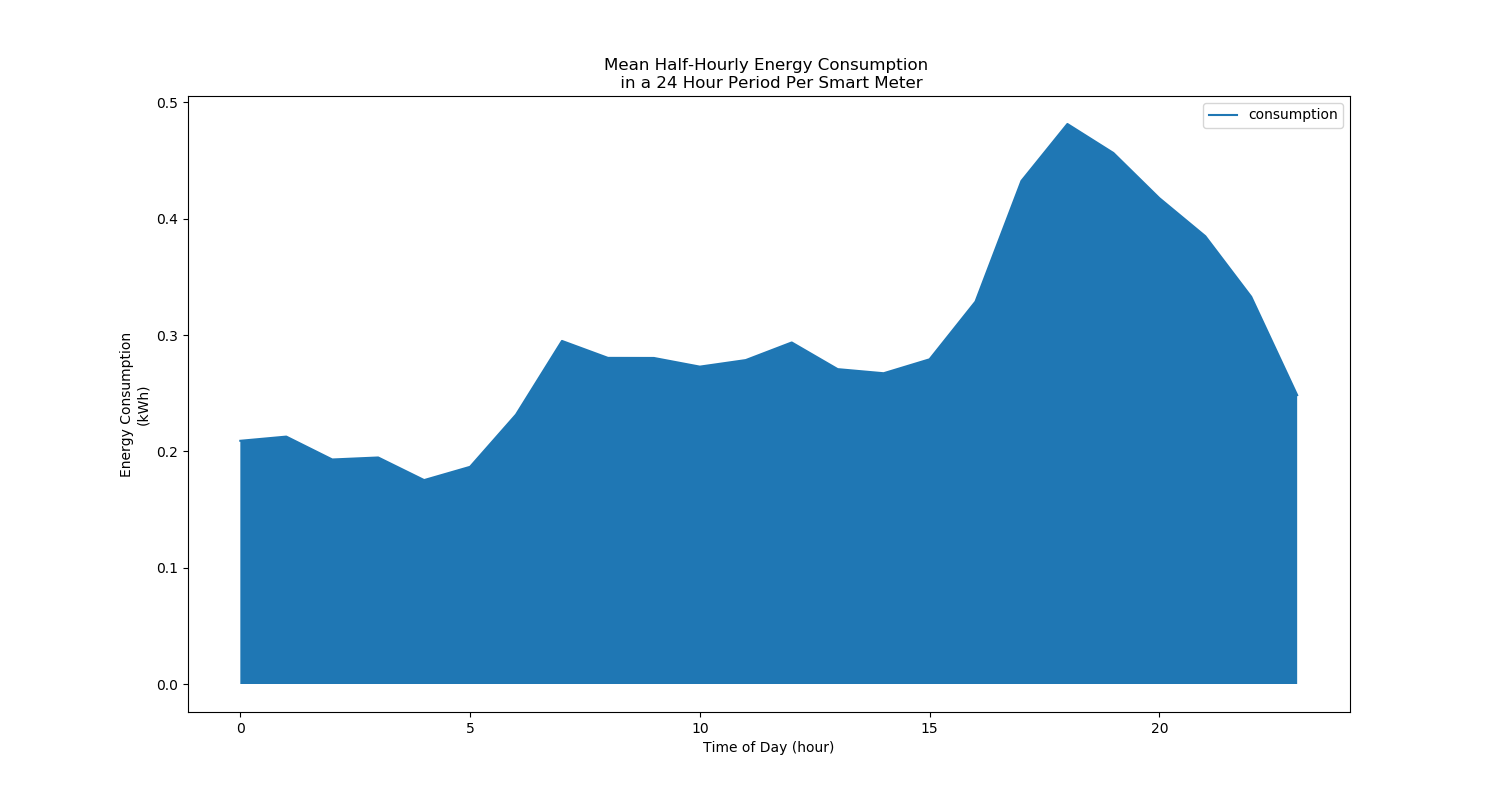
\includegraphics[width=1\textwidth]{Figures/EDA_images/mean_consumption_one_day.png}
        \caption{Mean Consumption per 24 Hour Period Per Smart Meter}
        \label{fig:Daily Consumption}
        \end{figure}
        
        Apart from looking at energy consumption values per time period, we can also investigate consumption values for the unique smart meter ANON\_IDs. In fig.3.3. we see the histogram generated to represent the frequency of mean energy consumption per half-hour per smart meter. This 'chunk' of data contains 295 unique ANON\_IDs, the mean half-hourly energy consumption is 0.281 kWh compare that to the median value of 0.250 kWh backup up the observed positive skew. The minimum is 0.0265 kWh compared the maximum value of 1.385 kWh representing a range of 1.3585 kWh. Fig.3.4. shows a box plot of the mean energy consumption per 30 minute interval per device. Here we there is an interquartile range (IQR) of 0.1965 kWh (0.1534 to 0.35 kWh). We can also observe a number of potential outliers above the $Q_3 + 1.5IQR$ value represented by the whisker.
        
        \begin{figure}[H]
        \centering     
        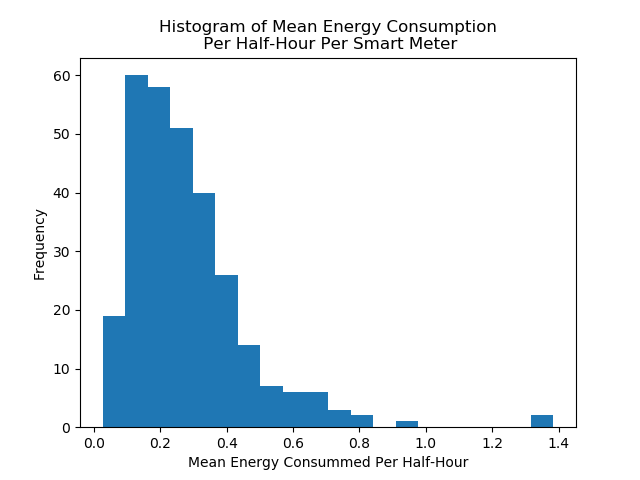
\includegraphics[width=1\textwidth]{Figures/EDA_images/mean_consumption_histogram.png}
        \caption{Histogram of Mean Consumption by ANON\_ID}
        \label{fig:Daily Consumption}
        \end{figure}
        
        \begin{figure}[H]
        \centering     
        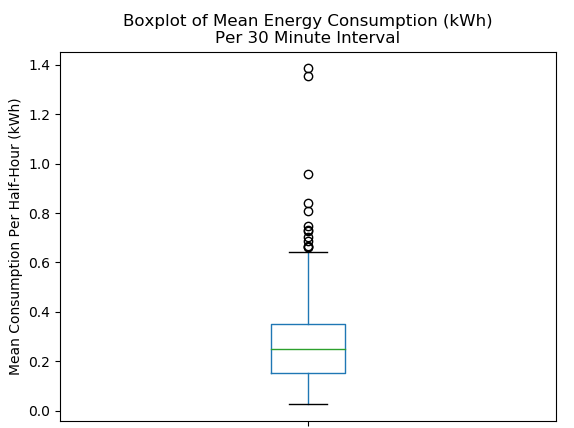
\includegraphics[width=0.75\textwidth]{Figures/EDA_images/mean_consumption_boxplot.png}
        \caption{Boxplot of Mean Consumption by ANON\_ID}
        \label{fig:Daily Consumption}
        \end{figure}
        
        These outliers may be indicative of a potential cluster, the distribution fig.3.3. shows that we have a narrow distribution, the standard distribution of the sample is 0.1827 kWh. If we were to translate that to clustering based on mean energy consumption we could expect to see a large cluster of low energy consumption dwellings with a centroid close to the median, a comparatively lower number of medium energy with a centroid approximately in the 0.5 to 0.8 kWh range and a third cluster with high energy usage. This outlines a point made in section 2.3.1. on limitations of k-means clustering which expects clusters of equal or similar size.
        
        \subsection{LAD 2011 UK Names and Codes} \\
        This data set contains Local Authority Districts (LAD) names and codes.
        
        \subsection{Geographic Data}
        \subsubsection{Description of Variables}
        \\
        This file is in XLSX format. This data set contains geographic data (Government Office Region and Local Authority) and ACORN segmentation data which can be linked to the consumption data via an anonymised household ID. ACORN is a segmentation tool which categorises the UK's population into demographic types. ACORN segments households, postcodes and neighbourhoods into 6 categories, 18 groups and 62 types. The following table outlines the variables contained within the Geographies data set:
        
        \begin{center}
            \begin{tabular}{|l |l|}
            \hline
             \textbf{Variable Name} & \textbf{Description} \\
             \hline\hline
             ANON\_ID & Integer case identifier (unique, not null, \\& use to link records in the other files) \\ 
             \hline
             eProfileClass & Domestic electricity profile class (1 or 2) \\
             \hline
             fuelTypes & Fuel Type - ElecOnly, GasOnly, or dual \\
             \hline
             ACORN\_Category & CACI Acorn category value \\
             \hline
             ACORN\_Group & CACI Acorn group value \\
             \hline
             ACORN\_Type & CACI Acorn type value \\
             \hline
             ACORN\_Code & CACI Acorn category, group and type values in one string \\
             \hline
             ACORN\_Description & English language description of CACI Acorn code \\
             \hline
             NUTS4 & Reflects the LAU1 areas to UK administrative \\&  geographies from 1$^{st}$ April 2010 \\
             \hline
             LACode & Reflects the UK Local Authority  boundaries that \\&  were in place on 21$^{st}$ June 2010\\
             \hline
             NUTS1 & Reflects the 12 NUTS1 areas to UK administrative \\& geographies from 1$^{st}$ April 2010\\
             \hline
             gspGroup & Electricity transmission network Grid Supply \\& Point Group code\\
             \hline
             LDZ & Gas transmission network Local Distribution Zone code\\
             \hline
             ELEC\_TOUT & Households containing an electricity meter \\& with a time of use tariff\\
             \hline
             GAS\_OUT & Households containing a gas meter with a time of use tariff\\
             \hline
            \end{tabular}
        \end{center}
        
        \subsubsection{Exploratory Data Analysis on Geographic Data Set}
        
        \begin{figure}[H]
        \centering     
        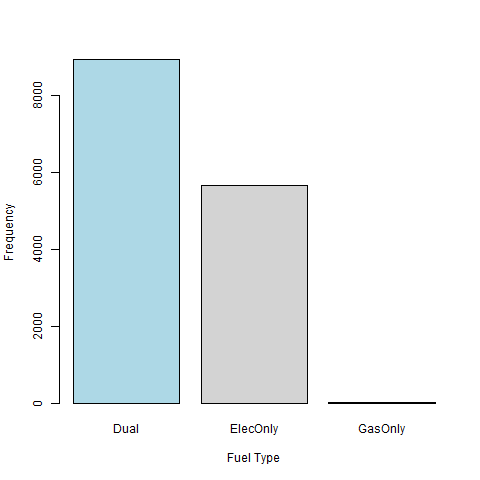
\includegraphics[width=1\textwidth]{Figures/EDA_images/fuel_table.png}
        \caption{Histogram of Mean Consumption by ANON\_ID}
        \label{fig:Daily Consumption}
        \end{figure}
        
        \begin{figure}[H]
        \centering     
        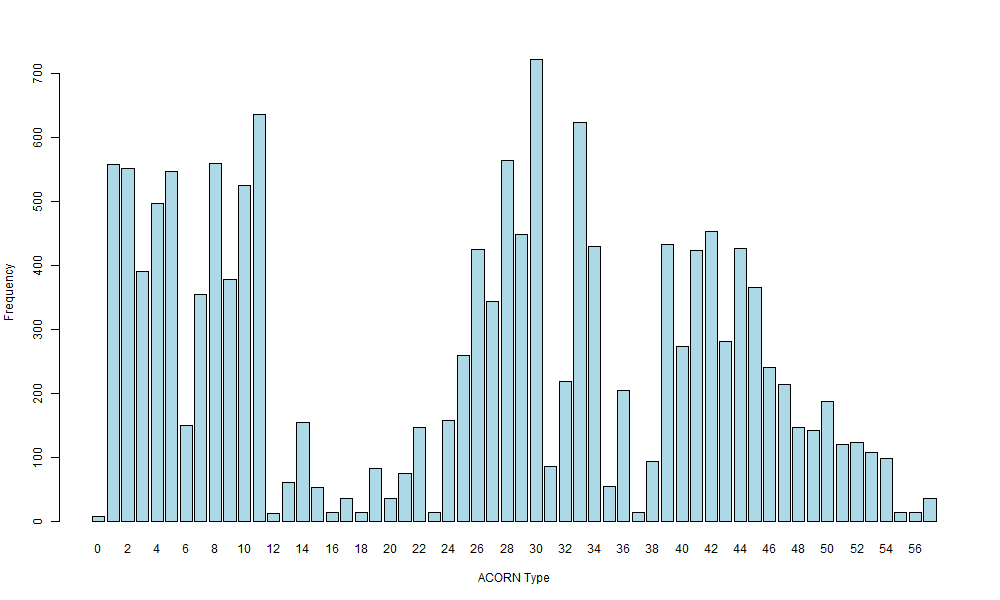
\includegraphics[width=1\textwidth]{Figures/EDA_images/acorn_type.png}
        \caption{Histogram of Mean Consumption by ANON\_ID}
        \label{fig:Daily Consumption}
        \end{figure}
        
        \begin{figure}[H]
        \centering     
        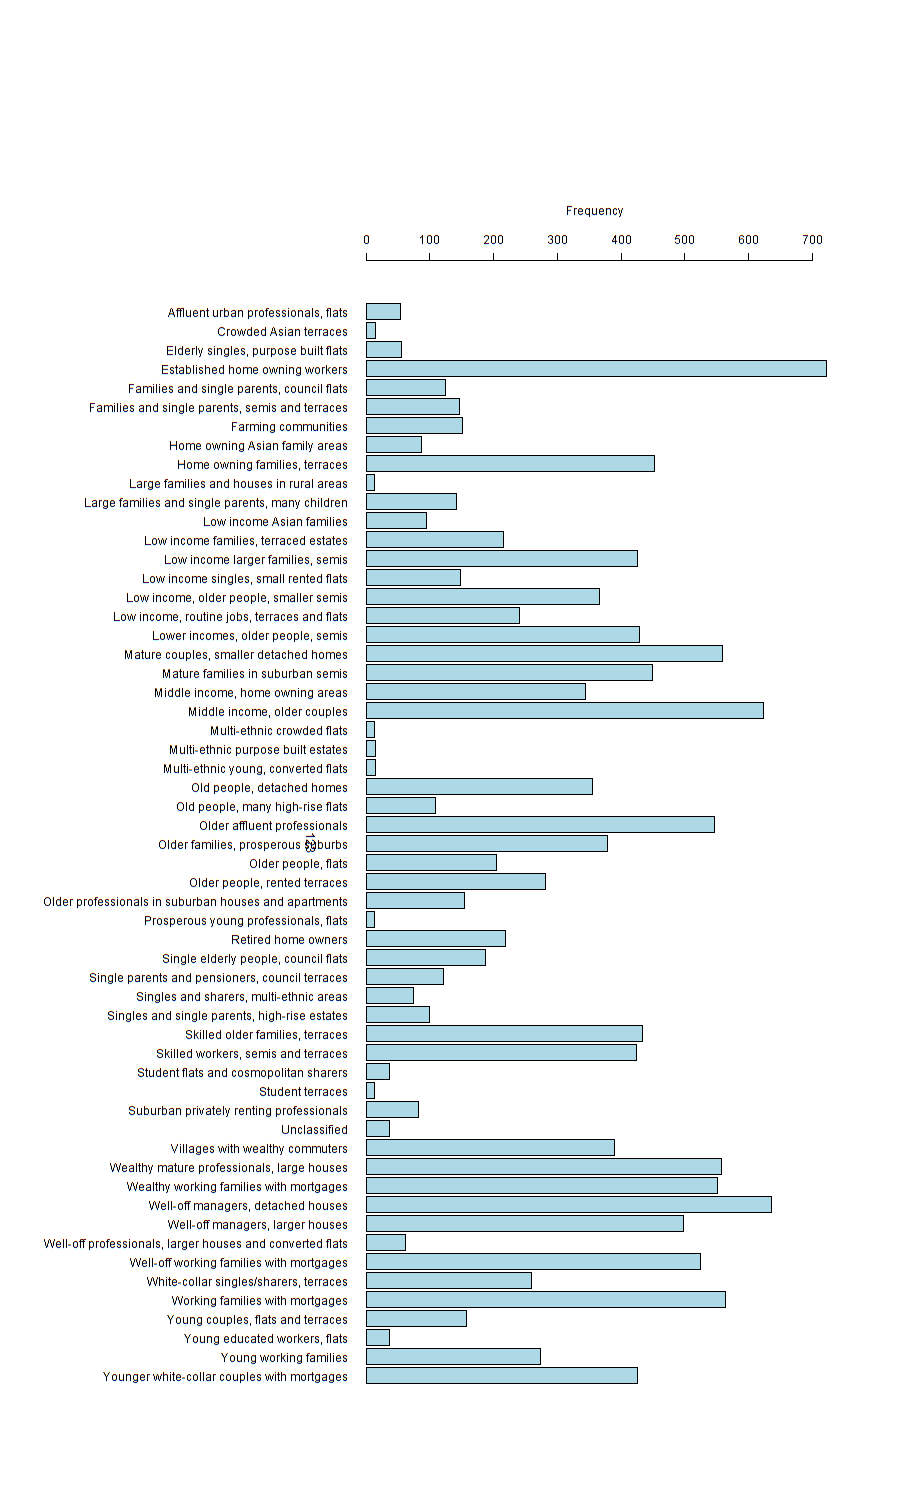
\includegraphics[width=1\textwidth]{Figures/EDA_images/acorn_description.png}
        \caption{Histogram of Mean Consumption by ANON\_ID}
        \label{fig:Daily Consumption}
        \end{figure}
        
        \subsection{Metadata} \\
        The metadata data set is a file containing explanatory descriptions of variables:
        
        \begin{left}
            \begin{tabular}{| l | l |}
            \hline
             \textbf{Variable Name} & \textbf{Description} \\
             \hline\hline
             Hhold\_ID & Integer case identifier (unique, not null, \\& use to link records in the other files) \\ 
             \hline
             firstAdvance & Date-Time of earliest electricity advance (halfhour
             precision) \\
             \hline
             fuelTypes & Fuel Type - ElecOnly, GasOnly, or dual \\
             \hline
             lastAdvance & Date-Time of latest electricity advance (halfhour
             precision) \\
             \hline
             days\_in\_range & Inclusive number of days between firstAdvance and
             lastAdvance \\
             \hline
             minAdvance & Lowest electricity advance value \\
             \hline
             maxAdvance & Highest electricity advance value \\
             \hline
             meanAdvance & Average electricity advance value \\
             \hline
             n\_expected & Number of advances expected based on
             days\_in\_range \\
             \hline
             n\_found & Number of advances available\\
             \hline
             pctFound & n\_expected/n\_found\\
             \hline
             TOUT & Time-of-use identifier\\
             \hline
            \end{tabular}
        \end{left}
        
        \subsection{Accompanying Documentation}\\
        PDF document containing all descriptions of data sets and variables contained within.
\section{Description of Process}
    In this section the workflow is described in detail and the challenges are outlined and discussed. It is as follows:
    \begin{itemize}
        \item Working With Large Data Sets
        \item Time Series and Dataframe Structure
        \item Clustering Time Series Data
        \item Pre-Process Geographic Data Set
        \item Build \& Tune The Random Forest Model
    \end{itemize}
    
\begin{figure}[H]
\centering     
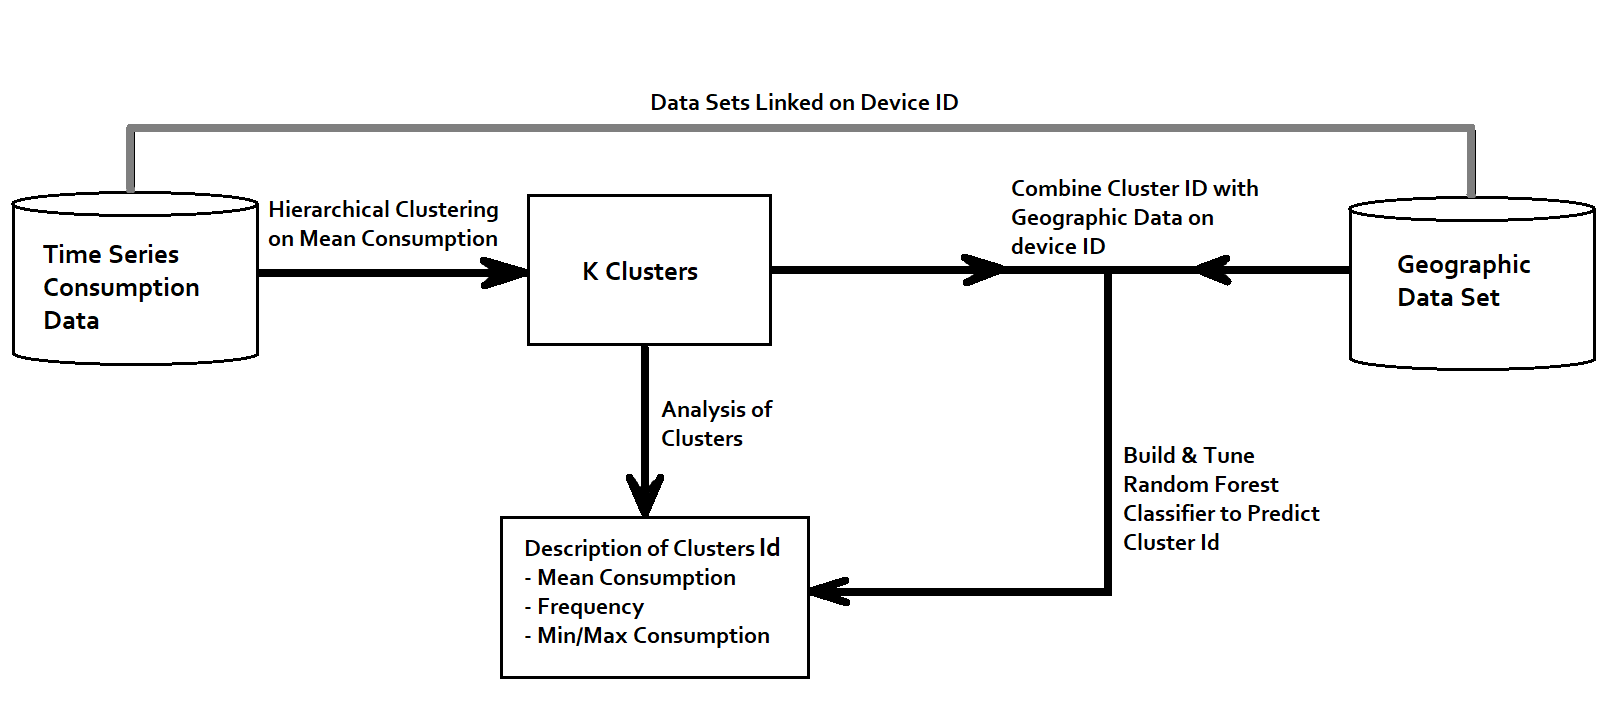
\includegraphics[width=1\textwidth]{Figures/workflow.png}
\caption{Work Flow of Project}
\label{fig:Dendrogram}
\end{figure} 
    
    \subsection{Working With Large Data Sets}
    As mentioned in section 3.1, the CSV file containing the half-hourly electrical energy consumption readings is 12GB in size. Reading this file into memory would likely cause a system failure due to the size of the file and limitations in RAM capacities. This is a common problem in working with Big Data and there are novel solutions available rather than just adding more RAM to the system. Some data sets can be terabytes in size so scaling up RAM isn't always cost efficient or even possible, a different approach this problem would be to read the file into memory in chunks. This would allow for a manageable portion of the data set to be read into memory, analysed and then dropped from memory, freeing up space for the next chunk and repeating this process until the entire data set has been processed. This would allow for a data set with $n$ number of observations to be partitioned into $k(\leq n)$ chunks such that $C = \{C_1, C_2, \dots, C_k\}$ (where each observation is assigned to one chunk) as to maximize the available memory limit. Maximizing the size of $k$ while not hitting the upper memory threshold would allow for shorter compute times as the number of iterations is inversely proportional to $k$. Another benefit to using this approach would be utilizing a distributed computing system. By breaking the data set down into chunks, the task of processing each one can be divided out into a number of different systems such that chunk $C_1$ is sent to system $S_1$, chunk $C_2$ sent to system $S_2$ and so forth. By working on the problem in parallel, the time taken to process the overall data set is reduced.
    
    \subsection{Time Series and Dataframe Structure}
    The original electrical consumption data set as mentioned in 3.1.1 is ordered by ADVANCEDATETIME. When this is partitioned into chunks, there is no prior knowledge of what ANON\_ID are contained within that chunk. The dataframe should be structured where each column is series of all the consumption values for a ANON\_ID. To do this, the chunk is looped through, new ANON\_IDs are identified and consumption values are appended to the corresponding ANON\_ID column and date-time row. The following table shows the final structure of the time series data for a chunk containing $j$ number of unique ANON\_IDs, $i$ number of date-time stamps ($t$) and energy consumption values $V$. Note that not all ANON\_IDs will be of the same length so there will be null values.

% HERE: TABLE DISPLAYING STRUCTURE OF TIME SERIES DATA FRAME    
\[ \begin{array}{l | cccccl}
\mbox{}         & anon\_id_1    & anon\_id_2    & anon\_id_3    & \quad ...     & \quad \rightarrow   & anon\_id_j \\
\hline
\mbox{t$_1$}    & V_{1,1}       &  V_{1,2}      &  V_{1,3}      & \quad ...     & \quad\rightarrow    &  V_{1,j}   \\
\mbox{t$_2$}    & V_{2,1}       &  V_{2,2}      &  V_{2,3}      &               &           & \\
\mbox{t$_3$}    & V_{3,1}       &  V_{3,2}      &  V_{3,3}      &               &           & \\
\mbox{...}      & ...           &               &               &\quad ...      &           & \\
\downarrow      & \downarrow    &               &               &               & \searrow  & \\
\mbox{t$_i$}    & V_{i,1}       &               &               &               &           & V_{i,j} \end{array}\]
    
    \subsection{Clustering Time Series Data}
    Now that the dataframe is in the correct structure, the time series data can be clustered. For clustering the SciPy library was imported, in order to perform hierarchical clustering the scipy.cluster.hierarchy.linkage() function was used. This function takes an input $y$ which may be in the form of a 1D condensed distance matrix or a 2D array of observation vectors, the latter is passed in. The following linkage methods are used to compute the distance $d(s,t)$ between two clusters $s$ and $t$. The algorithm begins with a forest of clusters that have yet to be used in the hierarchy being formed. When two clusters $s$ and $t$ from this forest are combined into a single cluster $u$, $s$ and $t$ are removed from the forest, and $u$ is added to the forest. When only one cluster remains in the forest, the algorithm stops, and this cluster becomes the root.
    
    A distance matrix is maintained at each iteration. The d[$i,j$] entry corresponds to the distance between cluster $i$ and $j$ in the original forest.

    At each iteration, the algorithm must update the distance matrix to reflect the distance of the newly formed cluster u with the remaining clusters in the forest.
    
    Suppose there are $|u|$ original observations $u[0],\dots, u[|u| -1]$ in cluster $u$ and $|u|$ original objects $v[0], \dots, v[|v| -1]$ in cluster $v$. Recall $s$ and $t$ are combined to form cluster $u$. Let $v$ be any remaining cluster in the forest that is not $u$.
    
    The following are method is used for calculating the distance between the newly formed cluster $u$ and each $v$.
    
    \begin{equation}
d(u, v) = \sum_{ij} \frac{d(u[i], v[j])}{(|u| \times |v|)}
    \end{equation}\
    
    For all points $i$ and $j$ where $|u|$ and $|v|$ are the cardinalities of clusters $u$ and $v$, respectively. This is also called the UPGMA algorithm.
    
    The metric used to calculate the distance was discussed in section 2.3.3
    
    The scipy.cluster.hierarchy.fcluster() function is used to form flat clusters from the hierarchical clustering defined by the linkage matrix. The hierarchical clustering encoded with the matrix returned by the linkage function is passed into the function. The maximum number of clusters..
    All the ANON\_IDs in the chunk are assigned a cluster.
    
    % PREPROCESSING THE GEO DATA (INCLUDING CHECKING NAs)
    \subsection{Pre-processing The Geographic Data}
    The geographic data set will be used in combination with the results of the clustering process in order to build an RF model capable of classifying a domestic energy consumer's energy needs. Before we build the classifier, the existing geographic data must be pre-processed in order to improve the accuracy of the model.
    Firstly some of the variables are removed, ACORN\_Category, ACORN\_Group, ACORN\_Description and ANON\_ID either fall under the category of indicator variables or variables that are directly correlated to other variables and therefore these variables are removed. 
    
     % dummy variables
    Next the remaining variables are converted to dummy variables. A dummy variable takes on the values of 0 or 1 to indicated the absence or presence of some categorical effect that may be expected to shift the outcome, note this increases the number of variables from 10 to 304. The R Library called '\textit{Caret}' will be utilized to carry out further pre-processing. The caret package(short for Classification And REgression Training) contains functions to streamline the model training process for complex regression and classification problems. Using caret we're going to remove near-zero variance variables. These are variables which either have a single unique value or unique value that occur with very low frequencies, for a model such as random forest it can cause them to become unstable so we're going to remove them here. This reduced the dimension of the data set down from (14,621 $\times$ 304) to (14,621 $\times$ 28), a considerable drop in variables.
    
    % remove correlated features
    Next we're going to look at correlated explanatory variables. To do this we make a correlation matrix, we can see that there were 2 variables with almost perfect correlation. Before we remove the variables, we use descrCor to get an idea of the overall correlation, it shows an overall mean correlation of -0.01823. We next set a cut-off of 0.75 and remove any variables with a correlation higher than this. This drops the dimension of the data down to (14,621 $\times$ 15), however the overall mean correlation is now -0.03837 which is marginally higher. Despite the marginal increase in correlation, the removed correlated features are not added back into the data set, here we are favoring a reduced complexity model. Note we also checked the data for linear dependencies and found none.
    % centre and scale
    Now we can center and scale the data. To do this we use the preProcess() function provided in \textit{Caret}. The final steps are to add back the ANON\_ID which we removed in the beginning. We also will map the results of the clustering onto the ANON\_ID.
    
    
    \subsection{Build and Tune Classification Models}
    In this section we will build 3 different models on the pre-processed data sets. There models will be used to predict what mean energy consumption cluster a consumer belongs to. The 3 models we will build are the Random Forest Model (RF), Gradient Boosting Model (GBM) and Support Vector Machine Model (SVM).
    
    For each models we will automate the tuning process using the \textit{Caret} library. To do this we first setup the training/test split in order to evaluate the models for the tuning process. Here we chose a 25-75 split. To evaluate the models we us a cross-validation technique in order to reduce the variance between models. Additionally we don't specifically want to choose the model with the highest accuracy as that model may be over fitting. To implement Occam's razor into our evaluation process we are going to define our selection function to chose the model within 2\% of the best model with the \textit{simplest parameters}. The evaluation metric is going to be based on the accuracy of the model.
    
    \subsubsection{Random Forest Model}
    The tuning parameters for the RF model are as follows:
        % list tuning parameters
        \begin{center}
            \begin{tabular}{|l |l|}
            \hline
             \textbf{Parameter} & \textbf{Chosen Values} \\
             \hline\hline
             mtry & $\sqrt{n}$ where n = number of features in train set \\
             \hline
            \end{tabular}
        \end{center}
    
    \subsubsection{Gradient Boosting Model}
    The tuning parameters for the GBM model are as follows:
        % list tuning parameters
        \begin{center}
            \begin{tabular}{|l |l|}
            \hline
             \textbf{Parameter} & \textbf{Chosen Values} \\
             \hline\hline
             Interaction Depth & [1, 5. 9] \\
             \hline
             N.trees & 50 - 1,500 in steps of 50 \\
             \hline
             shrinkage & Held constant at 0.1 \\ 
             \hline
             n.minobsinnode & Held constant at 20 \\
             \hline
            \end{tabular}
        \end{center}
        
        \subsubsection{Support Vector Machine Model}
        The tuning parameters for the SVM model are as follows:
        % list tuning parameters
        \begin{center}
            \begin{tabular}{|l |l|}
            \hline
             \textbf{Parameter} & \textbf{Chosen Values} \\
             \hline\hline
             preProc & [center, scale] \\
             \hline
             Tune Length & Held constant at 8\\
             \hline
            \end{tabular}
        \end{center} % Design and Implementation

\chapter{Evaluation and Testing}
\section{Introduction}
This section will review the work undertaken in chapter 3: Design and Implementation. Chapter 3 broke the workflow down to 5 main headings, here 3 headings are discussed in relation to the outcome of the processes.

\section{Results of Clustering}
In section 3.2.3: Clustering Time Series Data, hierarchical clustering was performed. Here the maxcluster parameter in the fclusters() function was chosen to be 3. Why was 3 chosen? As it's unknown the true number clusters contained in the data set and as we're clustering on average consumption as the metric, it is assumed that the data set will be partitioned into low, medium and high energy consumers. The results of the hierarchical clustering can be shown in the form of the dendrogram below in fig 4.1. It shows the index of each ANON\_ID on the x-axis, and the distance metric on the y-axis. This graph shows how ANON\_IDs are paired with the most similar and how pairs then make up the new combined series. All ANON\_IDs were assigned a cluster ID to which will be used later for classification using a Random Forest model.
\begin{figure}
\centering     
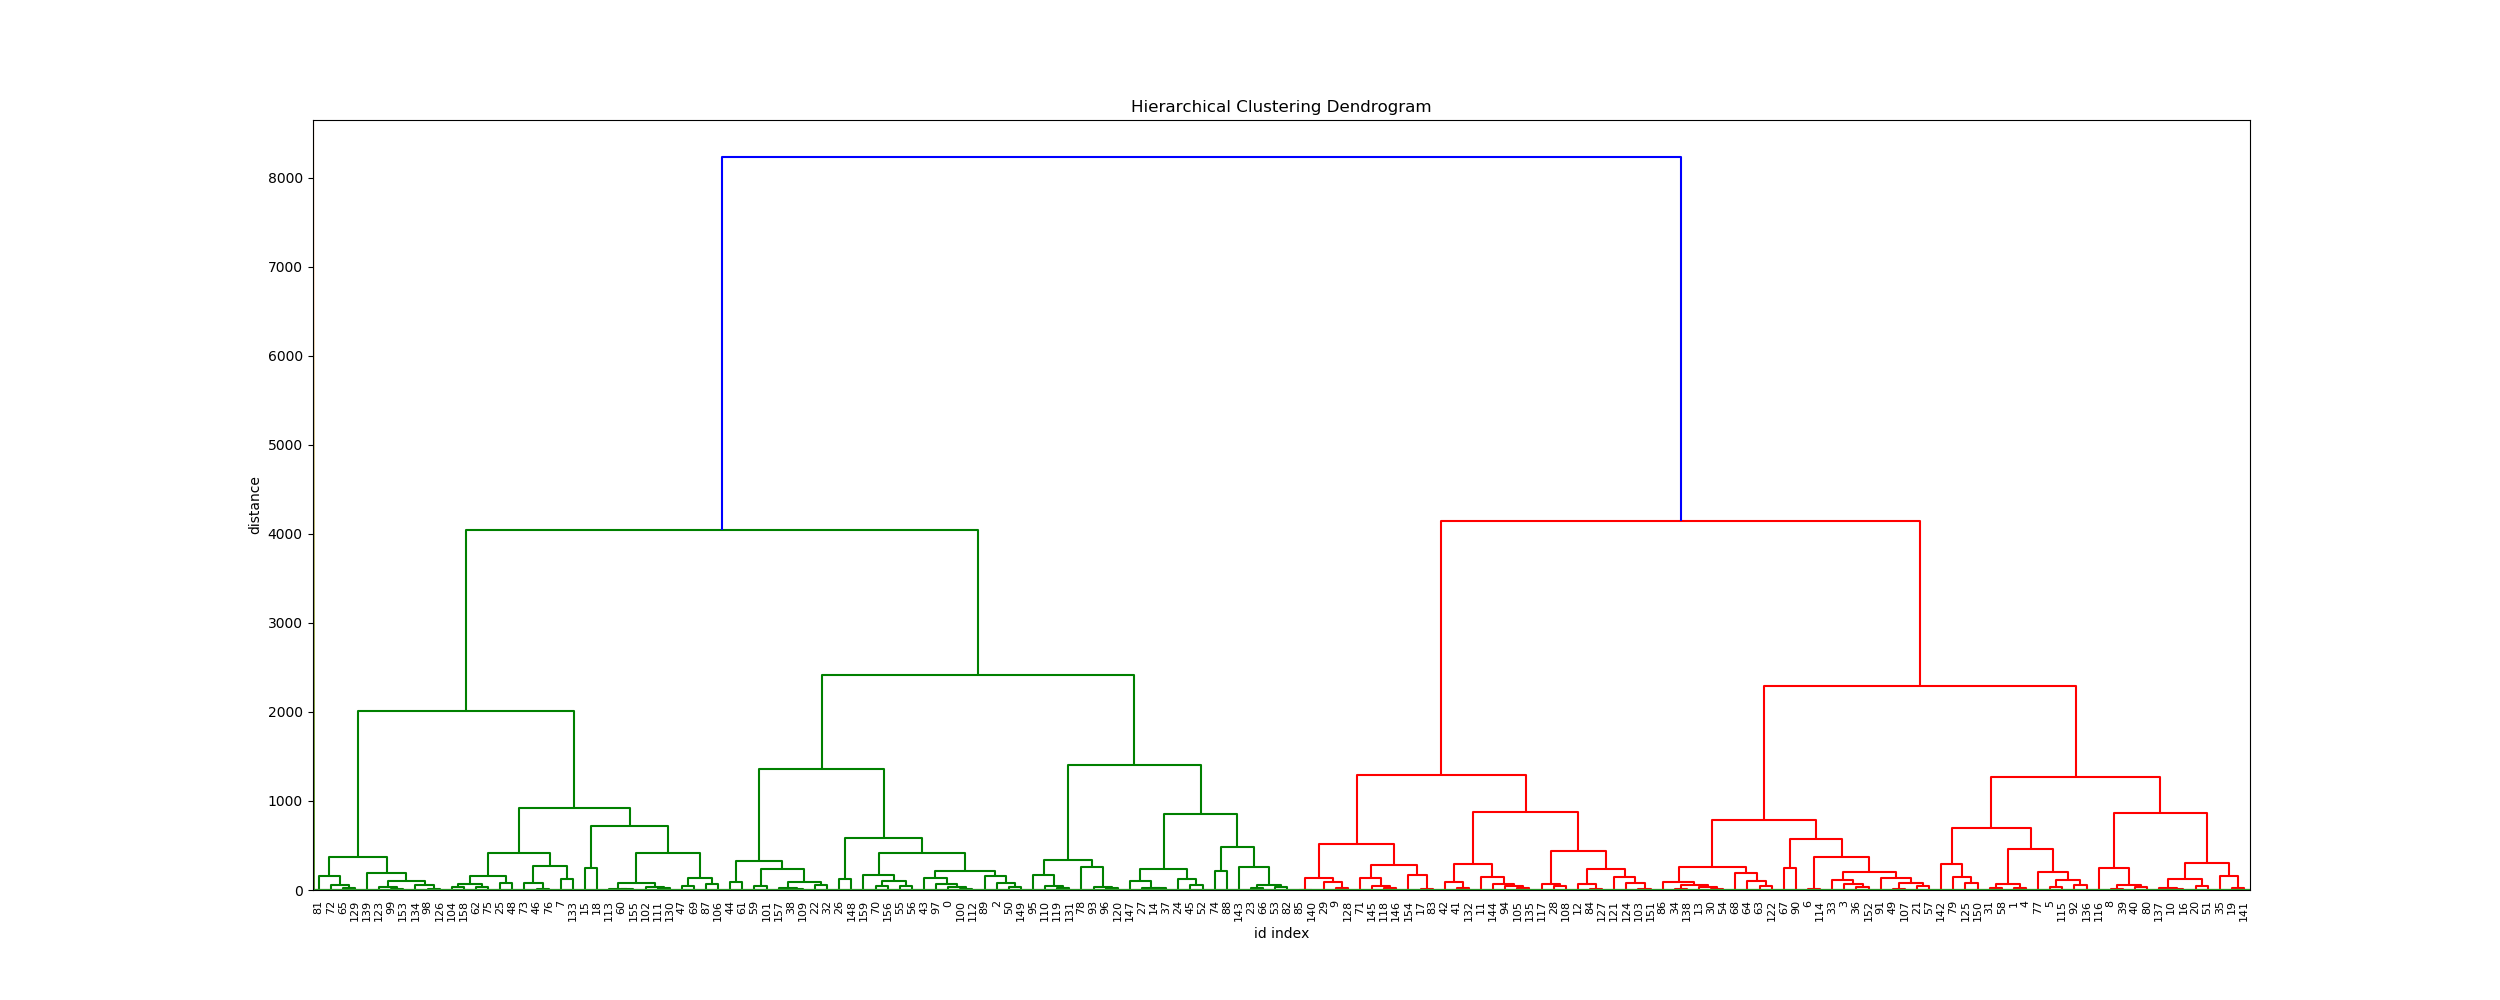
\includegraphics[width=1.5\textwidth, angle=90]{Figures/clusters_time_series.png}
\caption{Dendogram Generated from results of Hierarchical Clustering}
\label{fig:Dendrogram}
\end{figure} 

\subsection{Analysis of Clustering Results}
By assigning each ANON\_ID to a cluster then merging the time series consumption data along with the Geographies data set, data analysis can now be performed on the results of the clustering.

\begin{itemize}
    \item cluster frequency
    \item mean, min, max energy consumption per cluster
    \item correlation matrix, cluster with survey data
    \item further graphs with clusters \& survey data
\end{itemize}


\section{Results of Random Forest Model}
In this section, the performance of the random forest model built will be evaluated with reference various graphs generated. % Evaluation and Results

\chapter{Conclusions and Discussion}
As stated in the introduction, the goal of the project was to use consumer energy time series data to identify clusters of consumption patters and combine the results of which with geographic and demographic data to build a classifier to identify what cluster a consumer belongs to.

When we performed the clustering (on consumption data based on the mean energy consumption per half-hour) on the first chunk of data, we found 3 distinct clusters. These groups can be described as:
    \begin{itemize}
        \item Cluster 1: Low energy consumption and low variance
        \item Cluster 2: High energy consumption, medium variance
        \item Cluster 3: High energy consumption, high variance
    \end{itemize}
    
Each ANON\_ID in the chunk was then assigned to a cluster id. This then enabled us to merge the ANON\_ID and cluster id with the geographic data set. This new data set allowed us to analyse the geographic variables in relation to the cluster id. After pre-processing, the data set could now be passed into a Random Forest model to learn the important features from the geographic data set in order to predict what cluster id a ANON\_ID would belong to.

We saw in section 4.3, results of Random Forest Model, the accuracy of the model was somewhere in the 85-90\% range. However, as cluster group 1 represents ~87\% of the sample size, we could easily create a model with that level of accuracy just by assigning every observation to cluster group 1, which is essentially what this model is doing. The class imbalance as shown in fig.4.2. gives us some insight into why this is happening and also a potential solution. As cluster groups 2 \& 3 have a much lower frequency than cluster group 1, those cluster group observations may be up-sampled in the training set. By learning on a balanced training set it increases the signal of the minor class.


Our RF model, while work in progress, with further investigations could use demographic and geographic data set to predict new observations in geographic data set (new energy consumers/customers) without previous time series data. In order to accomplish the valuable use cases for this, as outlined in the introduction, further work must be done in the areas of time series pre-processing into and class balancing.

\begin{figure}[H]
\centering     
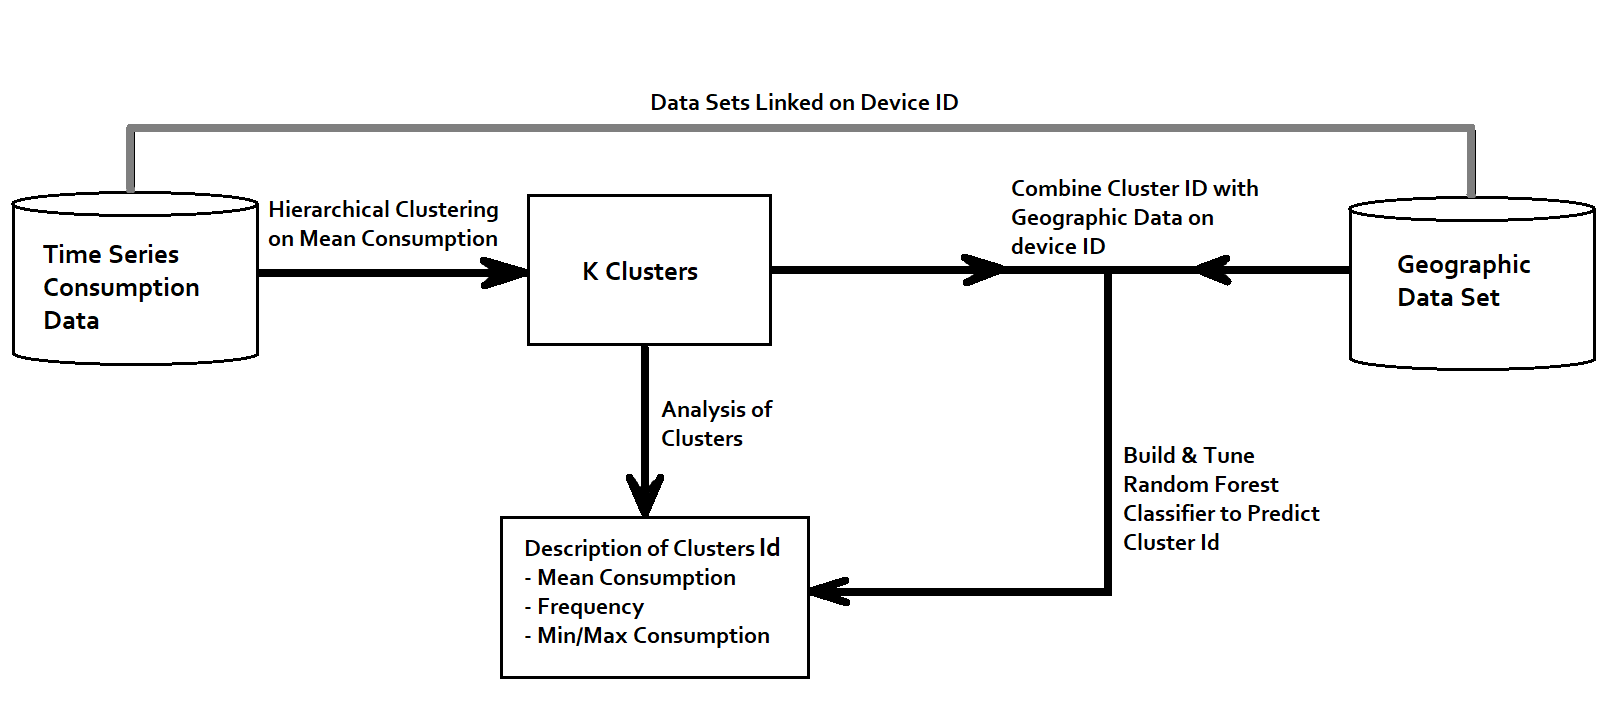
\includegraphics[width=1\textwidth]{Figures/workflow.png}
\caption{Work Flow Carried Out}
\label{fig:Dendrogram}
\end{figure} 

Instead of considering just one chunk of data as per this project, computational performance increases could be made by distributing multiple chunks to different systems and carrying out the same work flow in parallel. This would allow for a greater number of observations to be considered and would greatly enhance the computational efficiency over running this over just one system and by considering a greater number of observations, this would bring the sample mean closer to the true mean and therefore result in a better model.
 % Conclusions and Future Work

%% ----------------------------------------------------------------
\label{Bibliography}
\bibliographystyle{IEEEtranN}  % Use the "IEEE Transaction" BibTeX style for formatting the Bibliography
\bibliography{Bibliography}  % The references (bibliography) information are stored in the file named "Bibliography.bib"
\lhead{\emph{Bibliography}}  % Change the left side page header to "Bibliography"

%% ----------------------------------------------------------------
% Now begin the Appendices, including them as separate files

\addtocontents{toc}{\vspace{2em}} % Add a gap in the Contents, for aesthetics

\appendix % Cue to tell LaTeX that the following 'chapters' are Appendices

\chapter{Code Snippets}

Put appendix material in this section e.g. code snippets	% Appendix Title

\chapter{Wireframe Models} % Appendix Title

%\input{Appendices/AppendixC} % Appendix Title

\addtocontents{toc}{\vspace{2em}}  % Add a gap in the Contents, for aesthetics
\backmatter
\end{document}  % The End
%% ---------------------------------------------------------------- 